\documentclass[11pt,a4paper]{article}

% Packages
\usepackage[margin=2.5cm]{geometry}
\usepackage{microtype}
\usepackage{graphicx}
\usepackage{tikz}
\usetikzlibrary{shapes,arrows.meta,positioning,calc,fit,backgrounds,shadows.blur,decorations.pathmorphing,decorations.pathreplacing}
\usepackage{colortbl}
\usepackage{enumitem}
\usepackage{booktabs}
\usepackage{longtable}
\usepackage{hyperref}
\usepackage{xcolor}
\usepackage{fancyhdr}
\usepackage{titlesec}
\usepackage[most]{tcolorbox}
\usepackage{multicol}
\usepackage{amsmath,amssymb}
\usepackage{multirow}
\usepackage{setspace}
\usepackage{fontawesome5}
\usepackage{listings}

% Spacing
\setlength{\parskip}{3pt plus 1pt minus 1pt}
\setlength{\parindent}{0pt}

% Colors
\definecolor{primary}{HTML}{0E4D64}
\definecolor{secondary}{HTML}{137177}
\definecolor{accent}{HTML}{C84B31}
\definecolor{lightbg}{HTML}{E8F6F3}
\definecolor{defbg}{HTML}{FDF2E9}
\definecolor{greenhl}{HTML}{2E8B57}
\definecolor{purplehl}{HTML}{6C5B7B}
\definecolor{codebg}{HTML}{F4F6F7}

% Hyperref
\hypersetup{colorlinks=true, linkcolor=primary, urlcolor=secondary, citecolor=primary}

% Code/listing style
\lstset{
  backgroundcolor=\color{codebg},
  basicstyle=\ttfamily\small,
  keywordstyle=\color{primary}\bfseries,
  stringstyle=\color{greenhl},
  commentstyle=\color{gray},
  breaklines=true,
  frame=l,
  framerule=2pt,
  rulecolor=\color{secondary!40},
  xleftmargin=8pt,
  framexleftmargin=6pt,
  aboveskip=6pt,
  belowskip=6pt
}

\newcolumntype{L}[1]{>{\raggedright\arraybackslash}p{#1}}

% Header/Footer
\pagestyle{fancy}
\fancyhf{}
\fancyhead[L]{\small\textcolor{primary}{\textbf{Research Methods in IT --- MSIT}}}
\fancyhead[R]{\small\textcolor{primary}{Lecture Handout}}
\fancyfoot[C]{\small\thepage}
\renewcommand{\headrulewidth}{0.5pt}
\renewcommand{\footrulewidth}{0.3pt}

% Section formatting
\titleformat{\section}{\Large\bfseries\color{primary}}{\thesection}{0.6em}{}[\vspace{2pt}\titlerule]
\titleformat{\subsection}{\large\bfseries\color{secondary}}{\thesubsection}{0.5em}{}
\titleformat{\subsubsection}{\normalsize\bfseries\color{primary}}{\thesubsubsection}{0.5em}{}
\titlespacing*{\section}{0pt}{14pt}{8pt}
\titlespacing*{\subsection}{0pt}{10pt}{5pt}

% Custom boxes
\newtcolorbox{definitionbox}[1][] {
  enhanced,
  colback=defbg, colframe=orange!60!black,
  colbacktitle=orange!70!black, coltitle=white,
  title={\faIcon{book}~#1}, fonttitle=\bfseries,
  boxrule=0pt, leftrule=4pt, arc=2pt,
  shadow={1mm}{-1mm}{0mm}{black!15},
  top=4pt, bottom=4pt, left=8pt, right=8pt
}
\newtcolorbox{conceptbox}[1][] {
  enhanced,
  colback=lightbg, colframe=secondary,
  colbacktitle=secondary, coltitle=white,
  title={\faIcon{lightbulb}~#1}, fonttitle=\bfseries,
  boxrule=0pt, leftrule=4pt, arc=2pt,
  shadow={1mm}{-1mm}{0mm}{black!15},
  top=4pt, bottom=4pt, left=8pt, right=8pt
}
\newtcolorbox{alertbox}[1][] {
  enhanced,
  colback=red!4, colframe=accent,
  colbacktitle=accent, coltitle=white,
  title={\faIcon{exclamation-triangle}~#1}, fonttitle=\bfseries,
  boxrule=0pt, leftrule=4pt, arc=2pt,
  shadow={1mm}{-1mm}{0mm}{black!12},
  top=3pt, bottom=3pt, left=8pt, right=8pt
}
\newtcolorbox{examplebox}[1][] {
  enhanced,
  colback=green!4, colframe=greenhl,
  colbacktitle=greenhl, coltitle=white,
  title={\faIcon{code}~#1}, fonttitle=\bfseries,
  boxrule=0pt, leftrule=4pt, arc=2pt,
  shadow={1mm}{-1mm}{0mm}{black!12},
  top=3pt, bottom=3pt, left=8pt, right=8pt
}

\begin{document}

% Title
\begin{center}
\vspace*{0.5cm}
{\Huge\bfseries\textcolor{primary}{Research Methods in IT}}\\[8pt]
{\Large\bfseries\textcolor{primary}{Lecturer 101: Foundations for Academic and Applied Inquiry}}\\[16pt]
{\color{secondary}\rule{0.74\textwidth}{1.5pt}}\\[12pt]
{\Large\textsc{MSIT Lecture Handout}}\\[6pt]
{\large\textcolor{gray!70!black}{Course: Topics in IT \quad Program: MSIT}}\\[8pt]
{\normalsize\textcolor{gray!70!black}{Problem Identification \textbullet\ Research Design \textbullet\ Ethics \textbullet\ Analysis \textbullet\ Reporting}}
\vspace{0.3cm}
\end{center}

\tableofcontents
\newpage

%=============================================================
\section{Why Research Methods Matter in IT}
%=============================================================

\begin{definitionbox}[Research Methods in IT]
Research methods in IT are the structured principles and procedures used to identify a problem, collect trustworthy evidence, analyze findings, and produce defensible conclusions that can inform technology practice, policy, or innovation.
\end{definitionbox}

\begin{conceptbox}[Lecturer 101 View]
At introductory level, research methods are less about advanced statistics and more about disciplined thinking. A strong IT study begins with a clear problem, a justified method, ethical evidence collection, and conclusions that actually answer the research question.
\end{conceptbox}

\subsection{Why IT Professionals Need Research Skills}

\begin{itemize}[leftmargin=*]
  \item To evaluate whether a new tool, system, or framework actually works.
  \item To justify IT investments using evidence rather than opinion.
  \item To investigate user problems, security issues, or process inefficiencies.
  \item To contribute to academic, industry, and organizational knowledge.
  \item To communicate findings in a professional and reproducible way.
\end{itemize}

\subsection{Research as a Decision Process}

\begin{center}
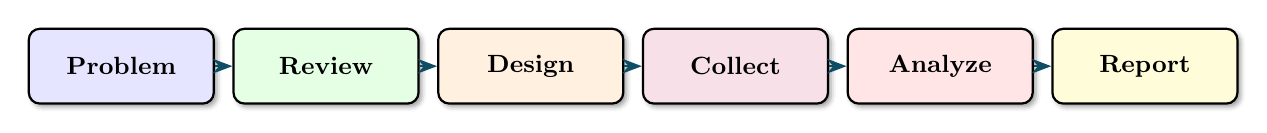
\begin{tikzpicture}[
  nodebox/.style={rectangle, draw, thick, rounded corners=4pt, minimum width=2.35cm, minimum height=0.95cm, align=center, font=\small\bfseries,
    blur shadow={shadow blur steps=3, shadow xshift=0.4mm, shadow yshift=-0.4mm}},
  arr/.style={-{Stealth[length=2.5mm]}, thick, primary}
]
  \node[nodebox, fill=blue!10] (problem) at (0,0) {Problem};
  \node[nodebox, fill=green!10] (review) at (2.6,0) {Review};
  \node[nodebox, fill=orange!12] (design) at (5.2,0) {Design};
  \node[nodebox, fill=purple!12] (collect) at (7.8,0) {Collect};
  \node[nodebox, fill=red!10] (analyze) at (10.4,0) {Analyze};
  \node[nodebox, fill=yellow!15] (report) at (13.0,0) {Report};
  \draw[arr] (problem) -- (review);
  \draw[arr] (review) -- (design);
  \draw[arr] (design) -- (collect);
  \draw[arr] (collect) -- (analyze);
  \draw[arr] (analyze) -- (report);
\end{tikzpicture}
\end{center}

\begin{longtable}{L{3.3cm}L{8.1cm}}
\toprule
\textbf{Stage} & \textbf{Key Question} \\
\midrule
Problem identification & What issue in IT needs investigation? \\
Literature review & What is already known and where is the gap? \\
Research design & Which method best answers the question? \\
Data collection & What evidence will be gathered and from whom? \\
Analysis & How will findings be interpreted? \\
Reporting & What conclusions, implications, and limits should be stated? \\
\bottomrule
\end{longtable}

%=============================================================
\section{From Topic to Research Problem}
%=============================================================

\subsection{Topic, Problem, and Gap}

\begin{definitionbox}[Research Problem]
A research problem is a specific and significant issue that requires systematic investigation. It is narrower than a broad topic and clearer than a general interest area.
\end{definitionbox}

\begin{examplebox}[From Broad Topic to Problem]
Broad topic: \emph{Cybersecurity awareness in universities}.

Better research problem: \emph{Despite repeated awareness seminars, phishing click rates among graduate students remain high, and the factors influencing unsafe email behavior are not clearly understood.}
\end{examplebox}

\subsection{Characteristics of a Good Research Problem}

\begin{itemize}[leftmargin=*]
  \item Clear and focused.
  \item Relevant to IT practice or policy.
  \item Researchable using available time and resources.
  \item Supported by observable evidence.
  \item Valuable enough to justify the study.
\end{itemize}

\subsection{Sources of Research Problems}

\begin{itemize}[leftmargin=*]
  \item Persistent system failures or usability complaints.
  \item Security incidents or policy non-compliance.
  \item Low adoption of digital platforms.
  \item Gaps in prior studies.
  \item Contradictory results in the literature.
\end{itemize}

\begin{alertbox}[Common Beginner Mistake]
Many students choose a technology instead of a problem. ``Blockchain'' is not a research problem. ``Barriers to blockchain adoption for academic credential verification in private universities'' is closer to a real research problem.
\end{alertbox}

%=============================================================
\section{Reviewing Related Literature}
%=============================================================

\subsection{What a Literature Review Does}

\begin{conceptbox}[Purpose of the Review]
The literature review shows what is already known, what methods others used, where findings disagree, and what gap your study intends to address.
\end{conceptbox}

\begin{itemize}[leftmargin=*]
  \item Defines concepts and variables.
  \item Identifies theories or models.
  \item Locates research gaps.
  \item Helps justify the chosen method.
  \item Prevents duplication of weak or outdated work.
\end{itemize}

\subsection{What to Read}

\begin{itemize}[leftmargin=*]
  \item Peer-reviewed journal articles.
  \item Conference papers in computing and IT.
  \item Standards, policies, and technical reports.
  \item Theses and dissertations when relevant.
  \item Credible institutional or industry publications.
\end{itemize}

\subsection{How to Organize the Review}

\begin{longtable}{L{3.1cm}L{8.3cm}}
\toprule
\textbf{Approach} & \textbf{What It Looks Like} \\
\midrule
Thematic & Group studies by themes such as usability, adoption, risk, or performance \\
Method-based & Group by survey, experiment, case study, interview, or mixed method \\
Chronological & Show how the field developed over time \\
Model-based & Compare studies using the same theory or framework \\
\bottomrule
\end{longtable}

\begin{examplebox}[Literature Matrix Idea]
A simple literature matrix may include: author, year, context, method, sample, key findings, and gap. This helps the researcher avoid reading articles in isolation.
\end{examplebox}

%=============================================================
\section{Research Questions, Objectives, and Hypotheses}
%=============================================================

\subsection{Research Questions}

Research questions guide the entire study. Good questions are specific, answerable, and aligned with the problem statement.

\begin{examplebox}[Sample Research Questions]
Study topic: learning management system adoption among graduate students.

Possible questions:
\begin{enumerate}[leftmargin=*]
  \item What factors influence graduate students' use of the learning management system?
  \item Is perceived ease of use associated with frequency of platform usage?
  \item What challenges do students report during remote access? 
\end{enumerate}
\end{examplebox}

\subsection{Research Objectives}

Objectives tell what the study intends to accomplish.

\begin{itemize}[leftmargin=*]
  \item \textbf{General objective:} broad purpose of the study.
  \item \textbf{Specific objectives:} measurable sub-goals that support the general objective.
\end{itemize}

\subsection{Hypotheses}

Hypotheses are testable statements, usually used in quantitative studies.

\begin{definitionbox}[Hypothesis]
A hypothesis is a tentative claim about the relationship between variables, stated in a form that can be supported or rejected through evidence.
\end{definitionbox}

\begin{examplebox}[Hypothesis Example]
\[H_0: \text{Perceived ease of use has no significant relationship with system usage frequency.}\]
\[H_1: \text{Perceived ease of use has a significant relationship with system usage frequency.}\]
\end{examplebox}

%=============================================================
\section{Research Designs Common in IT}
%=============================================================

\subsection{Quantitative Research}

Quantitative research focuses on numerical data, measurement, and statistical analysis.

\begin{itemize}[leftmargin=*]
  \item Surveys with scaled responses.
  \item Performance comparisons.
  \item Experiments and quasi-experiments.
  \item Log analysis and metrics evaluation.
\end{itemize}

\subsection{Qualitative Research}

Qualitative research focuses on meaning, experience, process, and context.

\begin{itemize}[leftmargin=*]
  \item Interviews with users or administrators.
  \item Focus group discussions.
  \item Observations of system use.
  \item Document or policy analysis.
\end{itemize}

\subsection{Mixed Methods Research}

Mixed methods combines numerical and narrative evidence in one study.

\begin{conceptbox}[Why Mixed Methods Fits IT]
Many IT problems have both technical and human dimensions. A survey may reveal how often a problem occurs, while interviews explain why it occurs.
\end{conceptbox}

\subsection{Common Designs at a Glance}

\begin{longtable}{L{2.8cm}L{3.1cm}L{5.5cm}}
\toprule
\textbf{Design} & \textbf{Best For} & \textbf{Typical IT Example} \\
\midrule
Survey & Describing attitudes or practices & User satisfaction with campus Wi-Fi \\
Experiment & Testing cause-effect claims & Comparing two authentication interfaces \\
Case study & Deep contextual investigation & Digital transformation in one university \\
Correlational & Examining relationships & Security awareness and password behavior \\
Mixed methods & Combining breadth and depth & LMS adoption rates plus student interviews \\
\bottomrule
\end{longtable}

%=============================================================
\section{Sampling and Participants}
%=============================================================

\subsection{Population and Sampling Frame}

The population is the full group of interest. The sampling frame is the practical list or source from which participants are selected.

\begin{examplebox}[Sampling Frame Example]
If the population is all MSIT students in a university, the sampling frame might be the official graduate student enrollment list for the current semester.
\end{examplebox}

\subsection{Probability and Non-Probability Sampling}

\begin{itemize}[leftmargin=*]
  \item \textbf{Probability sampling:} participants are selected with known chances, such as simple random sampling.
  \item \textbf{Non-probability sampling:} participants are selected through convenience, purposive choice, or availability.
\end{itemize}

\subsection{Examples of Sampling Techniques}

\begin{longtable}{L{3.0cm}L{8.4cm}}
\toprule
\textbf{Technique} & \textbf{Use Case} \\
\midrule
Simple random sampling & When a complete list of participants exists \\
Stratified sampling & When subgroups such as year level or role should be represented \\
Convenience sampling & When quick access matters more than strong generalization \\
Purposive sampling & When specialized participants are needed, such as IT administrators \\
Snowball sampling & When participants help identify others with similar expertise \\
\bottomrule
\end{longtable}

\subsection{Simple Response Rate Calculation}

\begin{examplebox}[Response Rate Example]
Suppose 150 questionnaires were distributed and 123 were returned.
\[
\text{Response rate} = \frac{123}{150} \times 100 = 82\%
\]
This is a useful descriptive statistic for reporting data collection quality.
\end{examplebox}

%=============================================================
\section{Instruments, Validity, and Reliability}
%=============================================================

\subsection{Research Instruments}

An instrument is the tool used to collect data.

\begin{itemize}[leftmargin=*]
  \item Questionnaire or survey form.
  \item Interview guide.
  \item Observation checklist.
  \item Test script, rubric, or performance log template.
\end{itemize}

\subsection{Validity}

Validity asks whether the instrument measures what it is supposed to measure.

\begin{itemize}[leftmargin=*]
  \item \textbf{Content validity:} items cover the concept adequately.
  \item \textbf{Construct validity:} items align with the underlying concept.
  \item \textbf{Face validity:} the instrument appears reasonable to experts or respondents.
\end{itemize}

\subsection{Reliability}

Reliability asks whether the instrument produces consistent results.

\begin{conceptbox}[Practical Meaning]
If a usability scale gives widely different results for the same situation without good reason, the instrument may have poor reliability.
\end{conceptbox}

\subsection{Likert-Scale Mean Example}

\begin{examplebox}[Mean Rating Example]
Suppose five respondents rate system usability on a 1--5 scale as follows:
\[
4,\ 5,\ 3,\ 4,\ 4
\]
The mean rating is
\[
\bar{x} = \frac{4+5+3+4+4}{5} = \frac{20}{5} = 4.0
\]
This suggests generally positive usability perception.
\end{examplebox}

%=============================================================
\section{Data Collection and Research Ethics}
%=============================================================

\subsection{Common Data Collection Methods}

\begin{itemize}[leftmargin=*]
  \item Online or printed surveys.
  \item Semi-structured interviews.
  \item Focus group discussions.
  \item System usage logs and audit trails.
  \item Controlled task performance observations.
\end{itemize}

\subsection{Ethical Principles}

\begin{itemize}[leftmargin=*]
  \item Informed consent.
  \item Voluntary participation.
  \item Privacy and confidentiality.
  \item Data security and secure storage.
  \item Honesty in reporting and citation.
\end{itemize}

\begin{alertbox}[Ethics in IT Research]
IT research often involves digital traces, logs, or identifiable online behavior. A dataset that appears technical may still contain personal or sensitive information and must be handled carefully.
\end{alertbox}

\subsection{Examples of Ethical Risks}

\begin{itemize}[leftmargin=*]
  \item Collecting login logs without proper permission.
  \item Recording interviews without explicit consent.
  \item Reporting findings in a way that identifies participants.
  \item Reusing a questionnaire without proper acknowledgment.
\end{itemize}

%=============================================================
\section{Data Analysis Basics for Lecturer 101}
%=============================================================

\subsection{Quantitative Analysis}

At introductory level, quantitative analysis often starts with descriptive statistics:

\begin{itemize}[leftmargin=*]
  \item Frequency and percentage.
  \item Mean and standard deviation.
  \item Ranking of factors.
  \item Correlation or basic hypothesis testing when appropriate.
\end{itemize}

\subsection{Qualitative Analysis}

Qualitative analysis often involves coding and theme development.

\begin{enumerate}[leftmargin=*]
  \item Read the responses carefully.
  \item Identify recurring ideas or phrases.
  \item Group them into codes.
  \item Merge related codes into themes.
  \item Interpret the themes in relation to the research questions.
\end{enumerate}

\subsection{Simple Frequency Example}

\begin{examplebox}[Percentage Example]
Suppose 48 out of 60 respondents say they use two-factor authentication.
\[
\text{Percentage} = \frac{48}{60} \times 100 = 80\%
\]
This indicates that most respondents report using two-factor authentication.
\end{examplebox}

\subsection{Interpreting Results}

\begin{conceptbox}[Interpretation Rule]
Do not stop at the numbers. Ask what they mean for IT practice. A high mean on usability should connect to design quality, support, adoption, or user productivity.
\end{conceptbox}

%=============================================================
\section{Writing the Research Proposal or Report}
%=============================================================

\subsection{Typical Sections}

\begin{longtable}{L{3.1cm}L{8.3cm}}
\toprule
\textbf{Section} & \textbf{Main Purpose} \\
\midrule
Introduction & Present the background and research problem \\
Review of literature & Show what is known and where the gap lies \\
Methodology & Explain design, participants, instruments, and analysis \\
Results & Present findings clearly and accurately \\
Discussion & Explain the meaning and implications of findings \\
Conclusion and recommendations & Summarize the study and suggest next steps \\
\bottomrule
\end{longtable}

\subsection{Good Academic Writing Practices}

\begin{itemize}[leftmargin=*]
  \item Write clearly and avoid unsupported claims.
  \item Align every section with the research questions.
  \item Use citations consistently.
  \item Report limitations honestly.
  \item Distinguish between findings, interpretation, and recommendation.
\end{itemize}

\begin{alertbox}[Weak Conclusion Pattern]
Avoid generic endings such as ``the system should be improved.'' A stronger conclusion specifies which part should be improved, based on which evidence, and why it matters.
\end{alertbox}

%=============================================================
\section{Mini Research Scenarios in IT}
%=============================================================

\subsection{Scenario 1: LMS Adoption}

Problem: Graduate students underuse the LMS despite institutional support.

Possible method: survey plus follow-up interviews.

Possible variables: perceived usefulness, ease of use, training quality, access reliability.

\subsection{Scenario 2: Phishing Awareness}

Problem: Staff continue clicking suspicious links after awareness campaigns.

Possible method: correlational survey and simulated phishing exercise.

Possible outputs: percentage of users who recognize phishing patterns, mean awareness score, thematic reasons for risky behavior.

\subsection{Scenario 3: Helpdesk Service Quality}

Problem: Users perceive IT support as slow and inconsistent.

Possible method: case study using helpdesk logs, survey ratings, and interviews.

\begin{examplebox}[How to Think Like a Researcher]
For each scenario, ask four things:
\begin{enumerate}[leftmargin=*]
  \item What is the exact problem?
  \item What evidence is needed?
  \item Which method fits that evidence?
  \item How will the findings help practice or policy? 
\end{enumerate}
\end{examplebox}

%=============================================================
\section{Quick Reference Summary}
%=============================================================

\begin{longtable}{L{3.4cm}L{7.8cm}}
\toprule
\textbf{Concept} & \textbf{Key Idea} \\
\midrule
Research problem & Specific issue requiring systematic investigation \\
Research gap & What prior work has not adequately answered \\
Research question & Direct question the study must answer \\
Objective & What the study intends to accomplish \\
Hypothesis & Testable statement about variables \\
Research design & Overall plan for collecting and analyzing evidence \\
Sampling & Selecting participants from a population \\
Validity & Accuracy of what an instrument measures \\
Reliability & Consistency of measurement \\
Ethics & Protection of participants and honest reporting \\
Analysis & Turning raw evidence into meaningful findings \\
\bottomrule
\end{longtable}

%=============================================================
\section{Key Takeaways and Review Questions}
%=============================================================

\subsection{Key Takeaways}

\begin{itemize}[leftmargin=*]
  \item Good IT research begins with a real problem, not just a trendy technology.
  \item The literature review justifies the gap and sharpens the study.
  \item Research questions, objectives, and hypotheses must align.
  \item Method choice depends on the nature of the evidence needed.
  \item Reliable instruments and ethical practice are non-negotiable.
  \item Results should be interpreted for IT practice, not only reported as numbers or quotes.
\end{itemize}

\subsection{Review Questions}

\begin{enumerate}[leftmargin=*]
  \item What is the difference between a broad topic and a research problem?
  \item Why is a literature review necessary before collecting data?
  \item When is a hypothesis useful in an IT study?
  \item How do quantitative and qualitative designs differ?
  \item Why are validity and reliability both important?
  \item What ethical issues commonly arise in IT research?
  \item What makes a conclusion academically strong? 
\end{enumerate}

\begin{examplebox}[Short Reflection Task]
Choose one IT issue from your workplace, institution, or community. Write one problem statement, two research questions, one suitable design, and one ethical concern you would need to manage.
\end{examplebox}

\vfill
\begin{center}
{\large\textcolor{primary}{\textbf{End of Handout}}}\\[4pt]
{\small\textcolor{gray!70!black}{Research Methods in IT --- MSIT Program}}
\end{center}

\end{document}